%!Mode:: "TeX:UTF-8"

\section{Squid}

Squid Cache(简称为Squid)是HTTP代理服务器软件。Squid用途广泛的,可以作为缓存服务器,可以过滤流量帮助网络安全,也可以作为代理服务器链中的一环,向上级代理转发数据或直接连接互联网。Squid程序在Unix一类系统运行。由于它是开源软件,有网站修改Squid的源代码,编译为原生Windows版;用户也可在Windows里安装Cygwin,然后在Cygwin里编译Squid。
\begin{figure}[ht]
	\begin{center}
		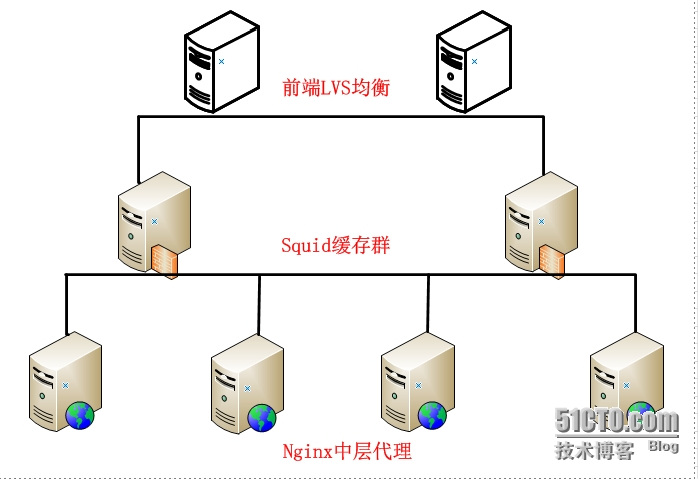
\includegraphics[keepaspectratio,width=0.3\paperwidth]{Pictures/Network/LvsPlusSquidPlusNginx.jpg}
		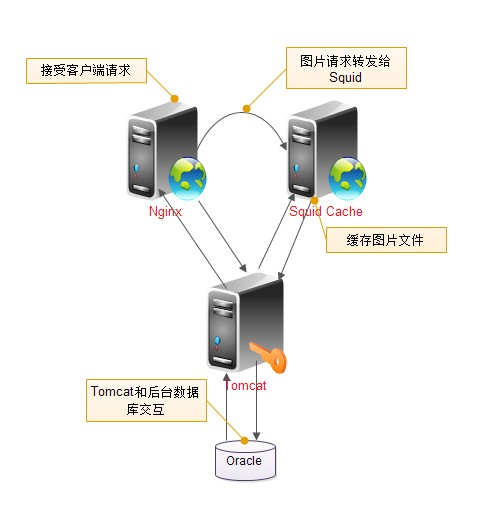
\includegraphics[keepaspectratio,width=0.3\paperwidth]{Pictures/Network/Nginx2Squid2Tomcat.jpg}
	\caption{Squid用作缓存服务器}
	\label{fig:LvsPlusSquidPlusNginx}
	\end{center}
\end{figure}


Squid的发展历史相当悠久,功能也相当完善。除了HTTP外,对于FTP与HTTPS的支持也相当好,在3.0测试版中也支持了IPv6。但是Squid的上级代理不能使用SOCKS协议。




\clearpage



